\documentclass[12pt]{amsart}
\usepackage[letterpaper, portrait, left = 1in, right = 1in, top = 1.2in, bottom=1.5in]{geometry} 
%\usepackage{setspace} \doublespacing
%\usepackage[letterpaper, portrait, margin=1.3in]{geometry}
\usepackage[table,xcdraw]{xcolor}
\usepackage{amssymb}
\usepackage{amsfonts}
\usepackage{longtable}
\usepackage{amsmath,amsthm}
\usepackage{enumitem}
\usepackage[utf8]{inputenc}
\usepackage{mathtools}
\usepackage{graphicx}
\usepackage{parskip}
\usepackage{multicol}
\usepackage{listings}
\usepackage[skip=0.25pt]{caption}
\usepackage[mathscr]{euscript}
\usepackage{quiver}
\setlength{\parindent}{0pt}
\usepackage{thm-restate}
\definecolor{vividburgundy}{rgb}{0.62, 0.11, 0.21}
\usepackage[driverfallback=hypertex,pagebackref=false,colorlinks,citecolor=vividburgundy]{hyperref}
\usepackage[capitalize]{cleveref}
%\usepackage[cmintegrals,cmbraces]{newtxmath}
%\usepackage{ebgaramond-maths}

%\usepackage{fourier}
%----------FONT OPTIONS----------
% sans-serif
%\usepackage[sfdefault]{FiraSans}
 %\usepackage[sfdefault]{roboto}
% \usepackage[sfdefault]{noto-sans}
%\usepackage[default]{sourcesanspro}

% serif
%\usepackage{CormorantGaramond}

%\usepackage{charter}
\usepackage[T1]{fontenc}
\usepackage{cleveref}
\definecolor{dg}{RGB}{10, 100, 10}
\setlength{\parindent}{0in}
\renewcommand{\qed}{$\hfill\blacksquare$}
% \newtheoremstyle{style}{2pt}{1pt}{\normalfont}{}{\bfseries}{\\}{0cm}{}
% \theoremstyle{style}
\newtheorem{lemma}{Lemma}[section]
% \newtheorem{lemma}{Lemma}
\newtheorem{thm}[lemma]{Theorem}
\newtheorem{prop}[lemma]{Proposition}
\newtheorem{cor}[lemma]{Corollary}
\newtheorem{conj}[lemma]{Conjecture}
\newtheorem{cl}[lemma]{Claim}
\newtheorem{rmk}{Remark}
\newtheorem{defn}[lemma]{Definition}
\newtheorem{qs}{Question}
\newtheoremstyle{styleS}{}{}{\color{dg}}{}{\color{dg}\bfseries}{. }{0cm}{}
\theoremstyle{styleS}
\newtheorem*{sol}{Solution}
\newtheoremstyle{style1}{}{}{\normalfont}{}{\bfseries}{. }{0cm}{}
\theoremstyle{style1}
\newtheorem{prob}{Problem}[section]
\newtheorem*{prb}{Problem}
\newtheoremstyle{style2}{1pt}{4pt}{\normalfont}{}{\itshape}{. }{0cm}{}
\theoremstyle{style2}
\newtheorem{ex}[lemma]{Example}
\newtheorem*{pf}{Proof}

\newcommand{\norm}[2]{
\left\lVert #1 \right\rVert_{#2}
}
\usepackage{mathrsfs}
%\usepackage[table,xcdraw]{xcolor}
\usepackage{booktabs}
\usepackage{tikz}
\usetikzlibrary{matrix}
\renewcommand{\l}{\ell}


\newcommand{\fA}{{\mathfrak{A}}}   \newcommand{\fB}{{\mathfrak{B}}}
\newcommand{\fC}{{\mathfrak{C}}}   \newcommand{\fD}{{\mathfrak{D}}}
\newcommand{\fE}{{\mathfrak{E}}}   \newcommand{\fF}{{\mathfrak{F}}}
\newcommand{\fG}{{\mathfrak{G}}}   \newcommand{\fH}{{\mathfrak{H}}}
\newcommand{\fI}{{\mathfrak{I}}}   \newcommand{\fJ}{{\mathfrak{J}}}
\newcommand{\fK}{{\mathfrak{K}}}   \newcommand{\fL}{{\mathfrak{L}}}
\newcommand{\fM}{{\mathfrak{M}}}   \newcommand{\fN}{{\mathfrak{N}}}
\newcommand{\fO}{{\mathfrak{O}}}   \newcommand{\fP}{{\mathfrak{P}}}
\newcommand{\fQ}{{\mathfrak{Q}}}   \newcommand{\fR}{{\mathfrak{R}}}
\newcommand{\fS}{{\mathfrak{S}}}   \newcommand{\fT}{{\mathfrak{T}}}
\newcommand{\fU}{{\mathfrak{U}}}   \newcommand{\fV}{{\mathfrak{V}}}
\newcommand{\fW}{{\mathfrak{W}}}   \newcommand{\fX}{{\mathfrak{X}}}
\newcommand{\fY}{{\mathfrak{Y}}}   \newcommand{\fZ}{{\mathfrak{Z}}}

\newcommand{\cA}{{\mathcal{A}}}   \newcommand{\cB}{{\mathcal{B}}}
\newcommand{\cC}{{\mathcal{C}}}   \newcommand{\cD}{{\mathcal{D}}}
\newcommand{\cE}{{\mathcal{E}}}   \newcommand{\cF}{{\mathcal{F}}}
\newcommand{\cG}{{\mathcal{G}}}   \newcommand{\cH}{{\mathcal{H}}}
\newcommand{\cI}{{\mathcal{I}}}   \newcommand{\cJ}{{\mathcal{J}}}
\newcommand{\cK}{{\mathcal{K}}}   \newcommand{\cL}{{\mathcal{L}}}
\newcommand{\cM}{{\mathcal{M}}}   \newcommand{\cN}{{\mathcal{N}}}
\newcommand{\cO}{{\mathcal{O}}}   \newcommand{\cP}{{\mathcal{P}}}
\newcommand{\cQ}{{\mathcal{Q}}}   \newcommand{\cR}{{\mathcal{R}}}
\newcommand{\cS}{{\mathcal{S}}}   \newcommand{\cT}{{\mathcal{T}}}
\newcommand{\cU}{{\mathcal{U}}}   \newcommand{\cV}{{\mathcal{V}}}
\newcommand{\cW}{{\mathcal{W}}}   \newcommand{\cX}{{\mathcal{X}}}
\newcommand{\cY}{{\mathcal{Y}}}   \newcommand{\cZ}{{\mathcal{Z}}}

\newcommand{\sA}{{\mathscr{A}}}   \newcommand{\sB}{{\mathscr{B}}}
\newcommand{\sC}{{\mathscr{C}}}   \newcommand{\sD}{{\mathscr{D}}}
\newcommand{\sE}{{\mathscr{E}}}   \newcommand{\sF}{{\mathscr{F}}}
\newcommand{\sG}{{\mathscr{G}}}   \newcommand{\sH}{{\mathscr{H}}}
\newcommand{\sI}{{\mathscr{I}}}   \newcommand{\sJ}{{\mathscr{J}}}
\newcommand{\sK}{{\mathscr{K}}}   \newcommand{\sL}{{\mathscr{L}}}
\newcommand{\sM}{{\mathscr{M}}}   \newcommand{\sN}{{\mathscr{N}}}
\newcommand{\sO}{{\mathscr{O}}}   \newcommand{\sP}{{\mathscr{P}}}
\newcommand{\sQ}{{\mathscr{Q}}}   \newcommand{\sR}{{\mathscr{R}}}
\newcommand{\sS}{{\mathscr{S}}}   \newcommand{\sT}{{\mathscr{T}}}
\newcommand{\sU}{{\mathscr{U}}}   \newcommand{\sV}{{\mathscr{V}}}
\newcommand{\sW}{{\mathscr{W}}}   \newcommand{\sX}{{\mathscr{X}}}
\newcommand{\sY}{{\mathscr{Y}}}   \newcommand{\sZ}{{\mathscr{Z}}}

\newcommand{\ta}{{\tilde{a}}}   \newcommand{\tb}{{\tilde{b}}}
\newcommand{\tc}{{\tilde{c}}}   \newcommand{\td}{{\tilde{d}}}
\newcommand{\te}{{\tilde{e}}}   \newcommand{\tf}{{\tilde{f}}}
\newcommand{\tg}{{\tilde{g}}}   
\newcommand{\ti}{{\tilde{i}}}   \newcommand{\tj}{{\tilde{j}}}
\newcommand{\tk}{{\tilde{k}}}   \newcommand{\tl}{{\tilde{l}}}
\newcommand{\tm}{{\tilde{m}}}   \newcommand{\tn}{{\tilde{n}}}
		         	\newcommand{\tp}{{\tilde{p}}}
\newcommand{\tq}{{\tilde{q}}}   \newcommand{\tr}{{\tilde{r}}}
\newcommand{\ts}{{\tilde{s}}}   
\newcommand{\tu}{{\tilde{u}}}   \newcommand{\tv}{{\tilde{v}}}
\newcommand{\tw}{{\tilde{w}}}   \newcommand{\tx}{{\tilde{x}}}
\newcommand{\ty}{{\tilde{y}}}   \newcommand{\tz}{{\tilde{z}}}

\newcommand{\red}{{\color{red}red}}
\newcommand{\blue}{{\color{blue}blue}}

\newcommand{\into}{\hookrightarrow}
\newcommand{\onto}{\twoheadrightarrow}
\newcommand\N{\ensuremath{\mathbb{N}}}

%\newcommand\L{\ensuremath{\mathbb{L}}}
\newcommand{\bP}{\mathbb{P}}
\newcommand\M{\ensuremath{\mathbb{M}}}
\newcommand\R{\ensuremath{\mathbb{R}}}
\newcommand\Z{\ensuremath{\mathbb{Z}}}
\renewcommand\O{\ensuremath{\emptyset}}
\newcommand\Q{\ensuremath{\mathbb{Q}}}
\newcommand\C{\ensuremath{\mathbb{C}}}
\newcommand{\K}{\ensuremath{\mathbb{K}}}
\newcommand\F{\ensuremath{\mathbb{F}}}
\newcommand{\aff}{\ensuremath{\mathbb{A}}}
\newcommand{\proj}{\ensuremath{\mathbb{P}}}
\newcommand{\dd}{\mathrm{d}}
\newcommand{\m}{\ensuremath{\mathfrak{m}}}
\newcommand{\p}{\ensuremath{\mathfrak{p}}}
\newcommand{\n}{\ensuremath{\mathfrak{n}}}
\renewcommand{\phi}{\varphi}
\renewcommand{\qedsymbol}{\ensuremath{\blacksquare}}
%\newcommand{\st}{\;|\;}
\newcommand{\st}{%
  \nonscript\;
  \ifnum\currentgrouptype=16
    \;\middle|\;
  \else
    \;|\;
  \fi
  \nonscript\;}
\newcommand{\ltr}{\par \noindent \framebox[1\width]{ $\implies$ } \hspace{.2cm}}
\newcommand{\rtl}{\par \noindent \framebox[1\width]{ $\impliedby$ } \hspace{.2cm} }
\newcommand{\abs}[1]{\left| #1 \right|}
\newcommand{\inner}[2]{\left\langle #1, #2 \right\rangle}
\newcommand{\E}[1]{\mathbb E\left[ #1 \right]}
\newcommand{\e}[1]{\exp\left( #1 \right)}
\renewcommand{\P}[1]{\mathbb P\left[ #1 \right]}
\newcommand{\Var}[1]{\text{Var}\left[ #1 \right]}
\newcommand*\circled[1]{\tikz[baseline=(char.base)]{
            \node[shape=circle,draw,inner sep=2pt] (char) {#1};}}
\newcommand{\ds}{\displaystyle}

\DeclareMathOperator{\sym}{Sym}
\DeclareMathOperator{\mds}{MDS}
\DeclareMathOperator{\Tor}{Tor}
\DeclareMathOperator{\Ext}{Ext}
\DeclareMathOperator{\adj}{adj}
\DeclareMathOperator{\Tr}{Tr}
\DeclareMathOperator{\GL}{GL}
%\DeclareMathOperator{\Tr}{Tr}
\DeclareMathOperator{\orbit}{Or}
\DeclareMathOperator{\stab}{Stab}
\DeclareMathOperator{\fix}{Fix}
\DeclareMathOperator{\re}{Re}
\DeclareMathOperator{\im}{Im}
\DeclareMathOperator{\ord}{Ord}
\DeclareMathOperator{\mspec}{mSpec}
\DeclareMathOperator{\spec}{Spec}
\DeclareMathOperator{\frob}{Frob}
\DeclareMathOperator{\id}{Id}
\DeclareMathOperator{\colim}{colim}
\DeclareMathOperator{\loc}{loc}
\DeclareMathOperator{\res}{Res}
\DeclareMathOperator{\rad}{rad}
\DeclareMathOperator{\Res}{Res}
\DeclareMathOperator{\diam}{diam}
\DeclareMathOperator{\arcsec}{arcsec}
\DeclareMathOperator{\arccot}{arccot}
\DeclareMathOperator{\len}{len}
\DeclareMathOperator{\area}{area}
\DeclareMathOperator{\vol}{vol}
\DeclareMathOperator{\ev}{ev}
\DeclareMathOperator{\sgn}{sgn}
\DeclareMathOperator{\supp}{supp}
\DeclareMathOperator{\diff}{d}
\DeclareMathOperator{\Dom}{Dom}
\DeclareMathOperator{\rk}{rank}
\renewcommand{\d}{\diff}
\let\oldend\endlinechar
\renewcommand{\endlinechar}{\oldend}
\newcommand{\open}{\underset{\text{open}}{\subset}}
\newcommand{\divides}{\mathbin{|}}
\newcommand{\set}[1]{\ensuremath{\left\{#1\right\}}}
\newcommand{\sett}{\coloneqq}
\newcommand*\isomap{%
  \xrightarrow{\raisebox{-0.9ex}[0ex][0ex]{$\sim$}}%
}
\renewcommand{\epsilon}{\varepsilon}
\newcommand{\fa}{~\forall~}
%\usepackage[nobottomtitles*]{titlesec}
\usepackage{titletoc}
%\titleformat{\section}[runin]
%{\normalfont\Large\bfseries}
%{}{0pt}{}%
%[\ifthenelse{\equal{\thesection}{0}}{\\\vspace*{0pt}}{\space\thesection}]
\newcommand{\sint}{\sin\theta}
\newcommand{\cost}{\cos\theta}
\newcommand{\tant}{\tan\theta}
\newcommand{\lb}{\left[}
\newcommand{\rb}{\right]}
\newcommand{\lp}{\left(}
\newcommand{\rp}{\right)}
\newcommand{\br}[1]{\lb#1\rb}
\newcommand{\pa}[1]{\lp#1\rp}
\usepackage{pdfpages}
\usepackage{fancyhdr}
	\pagestyle{fancyplain}
	\fancyhf{}
	\fancyhead[C]{\thepage}

\usepackage{wrapfig}
\usepackage{multicol}
\usepackage[breakable]{tcolorbox}
\usepackage{algorithm}
\usepackage{algpseudocode}
\usepackage[framed,numbered,autolinebreaks,useliterate]{mcode}
\usepackage{float}
%\usepackage{listings}
%\fontfamily{qcr}\selectfont 
%\usepackage[backend=bibtex]{biblatex}
\usepackage[
backend=biber,
style=alphabetic,%firstinits,
citestyle=ieee-alphabetic,
%natbib=true,
%uniquelist=false,
maxnames=10,
sorting=ynt
]{biblatex}
%\addbibresource{writeup/article/refs.bib}
%\title{\vspace{-1cm}}
\title{\textbf{CONVEX AND CONIC OPTIMIZATION}\\ Homework $6$}
\usepackage{quiver}
\usepackage[nobottomtitles*]{titlesec}
\usepackage{titletoc}
\titleformat{\section}[runin]
  {\normalfont\Large\bfseries}
  {}{0pt}{}%
  [\ifthenelse{\equal{\thesection}{0}}{\\\vspace*{0pt}}{\space\thesection}]
\author{{\Large NILAVA METYA} \\ 
\href{mailto:nilava.metya@rutgers.edu}{nilava.metya@rutgers.edu}\\
\href{mailto:nm8188@princeton.edu}{nm8188@princeton.edu}}
\date{May $2$, $2024$}
\newcommand{\pb}{\section{Problem}~\par}
\newcommand{\soln}{\subsection*{Solution}}
\newcommand{\conv}{\text{conv}}
\newcommand{\epi}{\text{epi}}
\usepackage{pdfpages}
\usepackage{fancyhdr}
	\pagestyle{fancyplain}
	\fancyhf{}
	\fancyhead[R]{\thepage}
\setlength{\columnsep}{1.2cm}
\newcommand{\fa}{~\forall}
\begin{document}

\maketitle

\pb

\begin{enumerate}[leftmargin=*]
\item Suppose you had a blackbox that given a 3SAT instance would tell you whether it is satisfiable or not. How can you make polynomially many calls to this blackbox to find a satisfying assignment to any satisfiable instance of 3SAT?
\item Suppose you had a blackbox that given a graph $G$ and an integer $k$ would tell you whether $G$ has a stable set of size larger or equal to $k$. How can you make polynomially many calls to this blackbox to find a maximum stable set of a given graph?
\end{enumerate}


\soln

\begin{enumerate}[leftmargin=*]
\item \boxed{\text{Sum, product in boolean expressions will denote \texttt{OR}, \texttt{AND} respectively.}}\\
Let $f$ be the blackbox. $f$ takes in a formula and outputs $1$ if satisfiable, and $0$ otherwise. \\
Let $S$ be a formula in CNF, with variables $x_{1},\cdots,x_{n}$. Treat $S$ as a polynomial in $x_{i}$'s. Assume $S$ is satisfiable, i.e., there are values $a_{1},\cdots,a_{n}\in\set{0,1}$ such that $S(a_{1},\cdots,a_{n})=1$. Often we denote $\pmb a = (a_{1},\cdots,a_{n})$. We will make $n$ calls to the blackbox. We find $\pmb a$ using $f$ as in \Cref{alg:sat}.

\begin{algorithm}
\caption{Finding SAT assignment using decision solving blackbox}\label{alg:sat}
\begin{algorithmic}
\Require Formula $S$ (which has a satisfiable assignment)
\Ensure Boolean numbers $a_{1},\cdots,a_{n}$ that satisfy $S$
\Procedure{FindSat}{$S$}
\State declare variables $y_{1},\cdots, y_{n}$
\For{$k = 1, \cdots, n$}
\State $y_{k}\gets x_{k}$
\If{$f\left(S\cdot\prod_{i=1}^{k}y_{i}\right)$}
	\State $a_{k} \gets 1$
\Else
	\State $y_{k}\gets \overline{x_{k}}$
	\State $a_{k} \gets 0$
\EndIf
\EndFor
\State \Return $\pmb a=(a_{1},\cdots,a_{n})$
\EndProcedure
\end{algorithmic}
\end{algorithm}

Let's justify the correctness via the following claims. The first statement in each bullet is a claim, followed by an explanation.
\begin{itemize}
\item \textbf{For each $i\in[n]$, at least one of $f(x_{i}\land S)$ or $f(\overline{x_{i}}\land S)$ is \texttt{True}.} If $a_{i}=1$ then $\left(x_{i}\land S\right)(\pmb a) = 1\cdot S(\pmb a) = 1$. 
If $a_{i}=0$ then $\left(\overline{x_{i}}\land S\right)(\pmb a) = 1\cdot S(\pmb a) = 1$.
\item \textbf{For any formula $\phi$, and a variable $x$ in it, $f(x\phi)=\texttt{True}$ iff $\phi$ has an assignment such that $x=1$}. Indeed if $f(x\phi)=\texttt{True}$ then there is some $\pmb c\in \set{0,1}^{N}$ (where $N$ is the number of variables in $\phi$) such that $\phi(\pmb c) = x(\pmb c) = 1$. On the other hand if $\pmb c$ is an assignment with $x(\pmb c) = 1 = \phi(\pmb c)$ then clearly $\pmb c$ satisfies $x\phi$. Note here that $x(\pmb c)$ is the coordinate of $\pmb c$ that corresponds to the variable $x$.
\item \textbf{At the end of the $k^{\text{th}}$ loop (for each $1\le k\le n$), $y_{1}\cdots y_{k}S$ is satisfiable with $y_{1}=\cdots=y_{k}=1$, where $S$ is the input to the above procedure.} (Inductively) assuming this is true till $t^{\text{th}}$ step, we note that the \textbf{if} statement in the $(t+1)^{\text{st}}$ iteration checks $f(S y_{1}\cdots y_{t} \cdot x_{t+1})$. We know that $Sy_{1}\cdots y_{t}$ is satisfiable with $y_{1}=\cdots =y_{t} = 1$. If $f(S y_{1}\cdots y_{t} x_{t+1})=1$ then $Sy_{1}\cdots y_{t}$ has a satisfiable assignment with $x_{t+1}=1$ (by the previous bullet) which is assigned to $a_{t+1}$ and $y_{t+1}$ is taken to be $x_{t+1}$ itself. 
If not, then (by first bullet) $Sy_{1}\cdots y_{t}  \overline{x_{t+1}}$ is satisfiable with $x_{t+1}=0$ which is assigned to $a_{t+1}$ again, but $y_{t+1}$ is taken to be $\overline{x_{t+1}}$. In either case, $S\cdot y_{1}\cdots y_{t+1}$ is satisfiable, by the end of the loop. The base case for $k=1$ is again true due to the previous bullet point.
\item \textbf{$y_{i} = a_{i}\cdot x_{i}+\overline{a_{i}}\cdot \overline{x_{i}}~\forall i\in[n]$}. This is clear by the construction. Note that this is exactly $\overline{a_{i}\texttt{ XOR }x_{i}}$.
\item \textbf{At the end, $y_{1}\cdots y_{n}S$ is satisfiable with the assignment  $x_{i}=a_{i}~\forall i$.} Using the third and fourth bullet above, $y_{i}=1$ exactly when $x_{i}=a_{i}$.
\end{itemize}
The above algorithm takes only $\mathcal O(n \cdot T(f))$ steps where $T(f)$ is the runtime of the blackbox $f$ (or $\mathcal O(n^{3} \cdot T(f))$ if we consider that it takes $\mathcal O(k)$ steps to form $y_{1}\cdots y_{k}S$ before passing it to $f$). Thus it's a polynomial-time reduction.

\item We have a decision problem solving submodule $\textsc{HasStab}(G,k)$ that takes input a graph $G$, an integer $k$ and outputs \texttt{True} if $G$ has a stable set of size (at least) $k$, and \texttt{False} otherwise. We also use a module $\textsc{Neigh}(G,v)$ which returns all neighbors of $v$ in $G$. 

\begin{algorithm}
\caption{Finding stable set using decision solving blackbox}\label{alg:cap}
\begin{algorithmic}
\Require Graph $G = (V,E)$ with $V=[n]$
\Ensure Maximal stable set in $G$
\Procedure{MaxStab}{$G$}
\State $n \gets$ number of vertices$, k\gets 0$
\For{$i = 1, \cdots, n$}\Comment{finding maximum stable set size}
\If{$\textsc{HasStab}(G,i)$}
	\State $k \gets i$
\EndIf
\EndFor
\State $S \gets \varnothing, t \gets k, G' \gets G$ \Comment{initialize a container for max stable set and make dummy variables}\For{$i = 1, \cdots, n$}\Comment{finding maximum stable set}
\State $G' \gets G'\smallsetminus \set{i}$
%\If{$i$ is not a vertex in $G'$}\State{continue}\EndIf
\If{($\texttt{NOT } \textsc{HasStab}(G',t)$)}
	\State append $i$ to $S$
	\State $t \gets t-1$
	\State $G' \gets$ $G'\smallsetminus \textsc{Neigh}(G',i)$
\EndIf
\EndFor
\State \Return $S$
\EndProcedure
\end{algorithmic}
\end{algorithm}

Let's show that this algorithm finds a maximal stable set. It is clear that the first \textbf{for} loop finds the size of maximal stable set $k$. From now on, when we say `loop', we refer to the second \textbf{for} loop. In the following enumerations, the first lines contains claims in bold, followed by a proof in the rest of the paragraph.

\begin{itemize}
\item \textbf{$S$ always remains stable}. Whenever $S$ is updated with, say, $v$, $G'$ is restricted to the non-neghbors of $v$, ensuring that every future update will only accept vertices in $S$ among non-neighbors of $v$. 
\item \textbf{At the start and end of every reiteration, $G'$ has a stable set of size $t$, for the respective current values}. (Inductively) assume true at the start of some loop. If removing $i$ from $G$ reduces the stable set number (by $1$ because one vertex is removed), which is exactly how $t$ is updated. If true at the end of some loop, then automatically true for the start of the next loop.
\item \textbf{At the end of every reiteration, $\abs S +t = k$}. This is because $t$ is updated to decrease by $1$ exactly when $S$ gets a new vertex.
\item \textbf{After the $i^{\text{th}}$ iteration, the only vertices remaining in $G'$ are a subset of $[n]\smallsetminus[i]$.} This is beacuse vertex $i$ is removed at the $t^{\text{th}}$ iteration.
\item \textbf{At the end of the iteration corresponding to $i=n$, the value of $t$ is $0$.} At the beginning of this iteration, $G'$ is either $\set{n}$ or $\varnothing$ (due to the previous bullet point), so that the only possible values of $t$ are $0,1$ (by the second bullet above). If $t=1$ then $G'=\set{n}$ so that only the \textbf{else} brach is executed and $t$ is updated to $0$. If $t$ was already $0$, then there is no update and the iteration ends with $t=0$. So at the end, $t=0$ anyway.
\end{itemize}

Due to the third and fifth bullet points above, the set $S$ we end with satisfies that $\abs S = k$ whence it has the same cardinality as a maximal stable set. The first bullet point shows that it is stable. Thus the algorithm outputs a maximal stable set.

Now coming to runtime. The number of steps is $\mathcal O(n\cdot T(\textsc{HasStab})+n\cdot T(\textsc{Neigh}))$ where $T(\textsc{HasStab})$ is the time to run the module $\textsc{HasStab}$ and $T(\textsc{Neigh})$ is the time to find neighbors of a vertex and remove it from the graph. The latter is clearly polynomial-time in terms of the input. Thus this is a poly-time reduction.

\end{enumerate}



\newpage

\pb

Consider a family of decision problems indexed by a positive integer $k$:
\subsection*{RANK-$k$-SDP}
\textbf{Input}: Symmetric $N\times N$ matrices $A_{1},\cdots,A_{m}$ with entries in $\Q$, scalars $b_{1},\cdots,b_{m} \in\Q$. \\
\textbf{Question}: Is there a real symmetric matrix $X$ that satisfies the constraints
\begin{equation}\label{rk1}\Tr(A_{i}X) = b_{i},i \in[m], X \succeq 0, \rk(X) = k?\end{equation}

\soln

\subsubsection*{RANK-$1$-SDP:}
First notice that a symmetric psd matrix $X\in S^{n}$ has rank $1$ iff it has the form $xx^{\top}$ for some $x\in \R^{n}\smallsetminus\set{0}$. So in the underlying problem, the constraints can be rewritten as $b_{i}=\Tr(A_{i}X) = x^{\top}A_{i}x\forall i\in[m]$ and $x\ne 0$. Thus it is clear that \begin{equation}\label{ee}\exists X\in S^{n} \text{ s.t. } X\succeq0,\Tr(A_{i}X) = b_{i}\forall i \in[m], \rk(X) =1\iff \exists x\in \R^{n} \text{ s.t. } x^{\top}A_{i}x = b_{i}\forall i\in[m], x\neq0.\end{equation}
We will show a reduction \textbf{STABLE-SET} $\longrightarrow$ \textbf{RANK-$1$-SDP}. Let $(G,k)$ be an instance of \textbf{STABLE-SET} where graph $G$ has edges $E$ and vertices $[n]$. Recall that this is same as feasibility of some $v\in \R^{n}$ satisfying $v_{i}(1-v_{i}) = 0~\forall i\in [n], v_{i}v_{j} = 0 ~\forall \set{i,j}\in E, \sum\limits_{i\in[n]} v_{i} \ge k.$\\
Since each $v_{i}\in \set{0,1}, \sum_{i\in[n]} v_{i}$ whence the last constraint is equivalent to the existence of some $s\in \R$ such that $\left(\sum\limits_{i\in[n]} v_{i}\right)^{2} - k^{2}=s^{2}$. So \textbf{STABLE-SET} is the feasibility of some $v,s$ subject to \begin{equation}\tag{(Q)}\label{Q}\begin{aligned}
v\in\R^{n}, &~s\in\R\\
v_{i}(1-v_{i}) &= 0~\forall i\in [n]\\
v_{i}v_{j} &= 0 ~\forall \set{i,j}\in E\\
\left(\sum_{i\in[n]} v_{i}\right)^{2}&=k^{2}+s^{2}.
\end{aligned}\end{equation}

\begin{cl}
Feasibility of \ref{Q} is equivalent to the feasibility of $v,c,s$ subject to 
\begin{equation}\tag{(QQ)}\label{QQ}\begin{aligned}
v\in\R^{n}, c\in\R, &~s\in \R\\
c^{2}&=1\\
v_{i}(c-v_{i}) &= 0~\forall i\in [n]\\
v_{i}v_{j} &= 0 ~\forall \set{i,j}\in E\\
\left(\sum_{i\in[n]} v_{i}\right)^{2}-s^{2}&=k^{2}.
\end{aligned}\end{equation}
\end{cl}
\begin{proof}
If $(v,s)$. is feasible to \ref{Q}, then $(v,1,s)$ is clearly feasible to \ref{QQ}.\\
Now suppose $(v,c,s)$ is feasible to \ref{QQ}. So each $v_{i}\in \set{0,c}\forall i\in[n]$. This means $k^{2}+s^{2} = \left(\sum_{}{i} v_{i}\right)^{2} = \left(\sum_{\substack{i\in[n]\\v_{i}= c}} v_{i}\right)^{2} = c^{2}\left(\sum_{\substack{i\in[n]\\v_{i}\ne 0}} 1\right)^{2} = \left(\sum_{\substack{i\in[n]\\v_{i}\ne 0}} cv_{i}\right)^{2} = \left(\sum_{i} cv_{i}\right)^{2}$. This shows that $(cv,s)$ is feasible to \ref{QQ}.
\end{proof}

Notice how all constraints in \ref{QQ} are polynomial expressions with only constant terms and homogeneous quadratic terms. This perfectly matches with what we want in the original problem using \cref{ee}. To get an instance of \textbf{RANK-$1$-SDP}, take: \begin{itemize}
\item The size of matrices $N = n+2$,
\item $Q = e_{n+1}e_{n+1}^{\top}$ and $q=1$,
\item $B_{i} = E_{i,n+1} - 2 e_{i}e_{i}^{\top}$ and $r_{i}=0$ for each $i\in[n]$
\item $A_{ij} = E_{ij} = e_{i}e_{j}^{\top} + e_{j}e_{i}^{\top}$ (which is the $N\times N$ matrix with $1$ in positions $(i,j),(j,i)$ and $0$ elsewhere), $b_{ij}=b_{ji}=0$ for each edge $\set{i,j}\in E$,
\item $T = \sum\limits_{1\le i,j\le n}e_{i}e_{j}^{\top} - e_{N}e_{N}^{\top}, b = k^{2}$.
\end{itemize}The above are clearly all rational.

Now consider the constraints on $x$ \begin{equation}\tag{(HQ)}\label{HQ}\begin{aligned}x&\in\R^{N}\\
x^{\top}Qx&=q\\
x^{\top}B_{i}x &= r_{i}\forall i\in[n]\\
x^{\top}A_{ij}x &= b_{ij}\forall \set{i,j}\in E \\
x^{\top}Tx &= b\end{aligned}\end{equation}
We show that this answers the same question as \textbf{STABLE-SET} gives on $(G,k)$.
\begin{cl}
\ref{QQ} is feasible iff \ref{HQ} is feasible.
\end{cl}
\begin{proof}
A solution $(v,c,s)\in \R^{n}\times \R\times\R$ of \ref{QQ} corresponds to a solution  $x=(v,c,s)\in \R^{N}$ of \ref{HQ}. \begin{align*}
x^{\top}Qx &= c^{2}  & 1 &= q\\
x^{\top}B_{i}x &= 2v_{i}c-2v_{i}^{2} &0 &=r_{i}\\
x^{\top}A_{ij}x &= 2v_{i}v_{j} & 0&=b_{ij}\\
x^{\top}Tx &= (v_{1}+\cdots+v_{n})^{2} - s^{2} & k^{2} &= b.
\end{align*}
Left column matches the LHS and right column matches the RHS of each constraint in \ref{QQ} and \ref{HQ}.
\end{proof}
Notice that every solution $x$ of \ref{HQ} is automatically nonzero because of the first constraint: $x_{n+1}^{2}=1$. 

The above shows that $G$ has a stable set of size (at least) $k$ iff \ref{HQ} is feasible, which is a problem of \textbf{RANK-$1$-SDP}. This completes the proof that \textbf{RANK-$1$-SDP} is NP hard because we showed a reduction from an NP hard problem.

\subsubsection*{RANK-$k$-SDP:}
We will show a reduction \textbf{RANK-$1$-SDP} $\longrightarrow$ \textbf{RANK-$k$-SDP} for $k\ge 2$. Indeed, consider an instance of \textbf{RANK-$1$-SDP} with inputs which are $N\times N$ matrices $A_{1},\cdots,A_{m}\in \Q^{N\times N}$ and scalars $b_{1},\cdots,b_{m}\in\Q$. Consider the following constraints: 
\begin{equation}\label{rkk}
\begin{aligned}
X\in& S^{N+k-1}\\
\rk(X) &= k\\
X&\succeq 0\\
\Tr(E_{ij} X) =&~ 0 ~\forall N < i < N+k, 1\le j\le N\\
\Tr(E_{ij} X) =&~ 0 ~\forall N < i< j< N+k\\
\Tr(E_{ii} X) =&~ 0 ~\forall N < i < N+k\\
\Tr(\tilde A_{i}X) =&~ b_{i}~\forall i \in[m].
\end{aligned}
\end{equation}
Here $\tilde A_{i} = \begin{bmatrix}A_{i}&0\\0&0\end{bmatrix}\in S^{N+k-1}$ obtained by putting appropriate number of $0$'s.

We discuss the above linear constraints one by one. On slight inspection, the above linear constraints deal with four different blocks of $X = \begin{bmatrix}A & B\\B^{\top}&C\end{bmatrix}$ where $A\in S^{N}, B\in \R^{N\times(k-1)}, C\in S^{k-1}$.
\begin{itemize}
\item $\Tr(E_{ij} X) = 0 ~\forall N < i < N+k, 1\le j\le N:$ here $E_{ij} = e_{i}e_{j}^{\top}+e_{j}e_{i}^{\top}$. This is just saying that $X_{ij} = X_{ji} = 0$ whenever $i>N$ and $j\in [N]$. In other words $B=0$.
\item $\Tr(E_{ij} X) = 0 ~\forall N < i< j< N+k:$  This looks at the block $C$ because $j>i>N$. The constraint says that all off-diagonal entries of $C$ are $0$, that is, $C$ is a diagonal matrix.
\item $\Tr(E_{ii} X) = 0 ~\forall N < i < N+k:$ This says that the diagonal entries of $C$ are all $1$. Using the previous point, $C$ is the identity matrix of size $(k-1)\times (k-1)$.
\end{itemize}

So this makes $X$ look like $\begin{bmatrix}A&0\\0&I_{k-1}\end{bmatrix}$. Note that $\rk(X) = \rk(A) + \rk(I_{k-1}) = \rk(A) + k-1$, whence $\rk(X) = k\iff \rk(A)=1$. Further $\begin{bmatrix}A&0\\0&I_{k-1}\end{bmatrix}\succeq0\iff A\succeq 0$ because eigenvalues of a block matrix formed of two blocks stacked diagonally is the union of the eigenvalues of the two individual blocks.

\begin{cl}
\ref{rk1} is feasible iff \ref{rkk} is feasible.
\end{cl}
\begin{proof}
From the above bullet points and the rank discussion, it is clear that a rank $1$ solution $A \succeq 0$ of \ref{rk1} corresponds to a rank $k$ solution $\begin{bmatrix}A&0\\0&I_{k-1}\end{bmatrix}\succeq 0.$
\end{proof}

This completes the proof that \textbf{RANK-$k$-SDP} is NP hard because we showed a reduction from an NP hard problem.


\newpage

\pb

A polynomial $p(x)\sett p(x_{1},\cdots,x_{n})$ is nondecreasing with respect to a variable $x_{i}$ if $\frac{\partial p}{\partial x_{i}}(x)\ge 0\forall x\in\R^{n}$. Show that the problem of deciding whether a degree-$d$ polynomial with rational coefficients is nondecreasing with respect to a particular variable (e.g., $x_{1}$) is
\begin{enumerate}[label=(\roman*)]
\item in P if $d<5$.
\item NP-hard if $d\ge 5$.
\end{enumerate}

\soln

Set $d=\deg(p)$. Here $p\in\Q[x_{1},\cdots,x_{n}]$. For short, denote $\partial_{i}p \sett \frac{\partial p}{\partial x_{i}}$. 

First note that $\deg(\partial_{i}(p)(x)) < d$ for each $i\in[n]$. This is because (fixing some $i\in[n]$) if $p(x) = x_{i}^{k}q_{k}(x_{-i}) + \cdots + x_{i} q_{1}(x_{-i}) + q_{0}(x_{-i})$ with all $q_{j}\in \Q[x_{-i}]$ ($x_{-i}$ denotes the vector with all variables in $x$ without $x_{i}$), then $d = \max\limits_{0\le j\le k}\set{j+\deg(q_{j})}$ whence $\deg (\partial_{i}p) = \max\limits_{1\le j\le k}\set{j-1+\deg(q_{j})} \le \max\limits_{0\le j\le k}\set{j-1+\deg(q_{j})} = d-1$ as a polynomial in $\Q[x]$.

The problem as mentioned, for each degree $d$, takes input $n$, the number of variables, the rational coefficients that make a polynomial, and an index $i$; and answers the question if the polynomial is non-decreasing in variable $x_{i}$. Denote the input size by $N$ - that is the number of coefficients till degree $d$. The degree $d$ of this polynomial can in fact be found in polynomial time in $N$. So there is a problem for each degree. Call it \textbf{MONO-d}.

\begin{enumerate}[label=(\roman*)]
\item We will show this by cases on degree of $d'=\deg(\partial_{i}p(x))$. Note that $d'\le 3$ if $d\le 4$.
\begin{itemize}
\item[$d=0:$] Then $\partial_{i}p = 0\ge 0$. So non-increasing. Thus we answered in constant time.
\item[$d'=0:$] Then $\exists b\in \Q$ such that $\partial_{i}p(x) = b$. Non-negativity of the rational constant $b$ can be checked in constant time.
\item[$d'=1:$] The required derivative looks like $\partial_{i}p(x) = b^{\top}x + c$ for some $b\in\Q^{n}\smallsetminus \set{0}, c\in\Q$. This is not everywhere non-negative because degree $1$.
\item[$d'=2$:] The required derivative looks like $\partial_{i}p(x) = \frac12x^{\top}Ax - b^{\top}x + c$ for some $A\in\Q^{n\times n},b\in\Q^{n}, c\in\Q$ and $A$ symmetric. Then:
\begin{itemize}
\item Say $A \not\succeq 0$. This is checked in $\mathcal{O}(n^{3})$ time. Then the function $\partial_{i}p$ is unbounded below: for example, along the direction of some eigenvector with negative eigenvalue.
\item So $A\succeq 0$ now. We have reduced to the problem of minimizing the convex function $\partial_{i}p(x)$ where $x\in\R^{n}$. Recall that if $x\in\R^{n}$ is a minima of this function then it's a critical point. Conversely if $x\in \R^{n}$ is a critical point, then $\nabla(\partial_{i}p)(x) = 0\implies \nabla(\partial_{i}p(x))^{\top}(y-x)\ge0\forall y\in\R^{n}$ whence it is a minima (convexity was needed here). If there is no $x\in\R^{n}$ such that $(Ax-b=)\partial_{i}p(x)=0$, then there is no minima and the problem is unbounded below. Otherwise assume there is a critical point $v \in\R^{n}$, that is, $Av=b$. In other words, $b$ is in the column span ($=$ row transpose span because $A$ is symmetric) of $A$. Then we claim every critical point takes the same objective. Indeed if $u$ is another critical point, then $Av = Au = b$ whence $A^{\top}(u-v)=A(u-v)=0$. Since $b$ is in the column span of $A$, $b^{\top}(u-v)=0$. But $\partial_{i}p(v) = -\frac12b^{\top}v+c = \frac12b^{\top}u+c=p(u)$. It follows that any critical point $v$ gives a global minima with value $-\frac12b^{\top}v+c$. 
\end{itemize} 
Thus our polynomial time algorithm is:
\begin{enumerate}
\item Differentiate $p(x)$ to get $A,b,c$ such that $\partial_{i}p(x) = \frac12x^{\top}Ax-b^{\top}x+c$.
\item Check if $A\succeq 0$. If not, conclude that $p$ is not non-decreasing wrt $x_{i}$ and {\tt{EXIT}} (because $\partial_{i}p$ is then unbounded below). Otherwise go to the next step.
\item Check if $b$ is in the column span of $A$. If not, conclude that $p$ is not non-decreasing wrt $x_{i}$ and {\tt{EXIT}} (because $\partial_{i}p$ is then unbounded below). Otherwise go to the next step.
\item Otherwise $\set{x\in\R^{n}\st Ax=b}\neq\varnothing$. Find a solution $\overline x$ to $Ax=b$. The objective $\partial_{i}p(\overline x)$ becomes $-\frac{1}{2}b^{\top}\overline x+c$. If this value is $\ge 0$, conclude that $p$ is non-decreasing wrt $x_{i}$ and {\tt{EXIT}}. Otherwise conclude that $p$ is not non-decreasing wrt $x_{i}$ and {\tt{EXIT}}.
\end{enumerate}
This is correct because of the above discussion. This runs in polynomial time in size of input because step (a) takes same number of steps as number of coefficients; step (b) takes $\mathcal{O}(n^{3}) \le \mathcal{O}(N^{3})$ steps; step (c) can be done in polynomial time (in $n$) again (say Gaussian elimination); and step (d) can again be done in polynomial steps in $n$. So overall, the number of steps this algorithm takes is polynomial in the input size $N$.
\item[$d'=3:$] So $\partial_{i}p(x)$ restricted to $\set{x\in\R^{n}\st x_{1}=x_{2}=\cdots=x_{n}}$ gives a $3-$degree polynomial in one variable which, we know from elementary theory, is unbounded below.
\end{itemize}
\item We'll now show a reduction \textbf{COPOS} $\longrightarrow$ \textbf{MONO-$d$} for $d\ge 5$, where \textbf{COPOS} takes input a matrix $M$ and decides whether it is copositive. Given an input $M\in\Q^{n\times n}$ to \textbf{COPOS}, we'll give the input $\ds p(x_{1},\cdots,x_{n+1})\sett x_{n+1} \left(\sum_{1\le i\le j\le n}M_{ij}x_{i}^{2}x_{j}^{2}\right) + x_{1}^{d}$ and variable index $n+1$ to \textbf{MONO-$d$}. This makes $\deg$ of the first term to be $5$ which is why we want $d\ge 5$. Then the following is immediate.
\begin{cl}
$M$ is copositive iff $p$ is non-decreasing wrt $x_{n+1}$.
\end{cl}
\begin{proof}
Note that $\ds\partial_{n+1}p(x) = \sum_{1\le i\le j\le n}M_{ij}x_{i}^{2}x_{j}^{2} = \begin{bmatrix}x_{1}^{2}\\\vdots\\x_{n}^{2}\end{bmatrix}^{\top}M\begin{bmatrix}x_{1}^{2}\\\vdots\\x_{n}^{2}\end{bmatrix}\ge 0$ for all $x\in\R^{n+1}$, iff $v^{\top}Mv\ge 0\forall v\in\R^{n} $ satisfying $v\ge 0$, iff $M$ is copositive.
\end{proof}
Since \textbf{COPOS} is known to be NP-hard, the above reduction shows that \textbf{MONO-$d$} is NP-hard.
\end{enumerate}

\newpage
\pb
\begin{enumerate}[leftmargin=*]
\item In the file \texttt{regression\textunderscore data.mat}, you are given $20$ points $(x_{i}, f_{i})$ in $\R^{2}$ where $(x_{i})_{i=1,\cdots,20}$ are the entries of the vector \texttt{xvec} and $(f_{i})_{i=1,\cdots,20}$ are the entries of the vector \texttt{fvec}. The goal is to fit a polynomial of degree $7$ \begin{equation}\label{pol} p(x) = c_{0} +c_{1}x+\cdots+c_{7}x^{7}\end{equation} to the data to minimize least square error: \begin{equation}\label{ls}\min_{c_{0},\cdots,c_{7}} \sum_{i=1}^{20}(f_{i}-p(x_{i}))^{2}.\end{equation} The data comes from noisy measurements of an unknown function that is a priori known to be nondecreasing (e.g., the number of calories you intake as a function of the number of Big Macs you eat).
\begin{enumerate}[label=(\alph*)]
\item If the underlying function is truly monotone and the noise is not too large, one may hope that least squares would automatically respect the monotonicity constraint. Solve (\ref{ls}) to see if this is the case. Plot the optimal polynomial you get and report the optimal value.
\item Resolve (\ref{ls}) subject to the constraint that the polynomial (\ref{pol}) is nondecreasing. Plot the optimal polynomial you get and report the optimal value.
\end{enumerate}
\item In the file \texttt{regression\_data.mat}, you are also given $30$ points $(x^{1}_{i} , x^{2}_{i} , g_{i})$ in $\R^{3}$ where $(x^{1}_{i})_{i=1,\cdots,30}$ are the entries of the vector \texttt{x1vec}, $(x^{2}_{i})_{i=1,\cdots,30}$ are the entries of \texttt{x2vec} and $(g_{i})_{i=1,\cdots,30}$ are the entries of the vector \texttt{gvec}. The goal in this case is to fit a polynomial of degree $4$: $$p\sett p(x_{1},x_{2}) = c_{0}+c_{1}x_{1} + c_{2}x_{2}+ c_{3}x_{1}^{2}+ c_{4}x_{1}x_{2}+c_{5}x_{2}^{2}+\cdots+c_{15}x_{2}^{4}$$ to the data to minimize least square error: \begin{equation}\label{ls2}
\min_{c_{0},\cdots,c_{15}} \sum_{i=1}^{30}(g_{i}-p(x_{i}))^{2}.
\end{equation}
\begin{enumerate}[label=(\alph*)]
\item Solve \ref{ls2} and plot the resulting polynomial together with the data points. Report the optimal value of the problem (denoted by $\eta^{*}$). Is the optimal polynomial convex?
\item Find a convex polynomial $p$ of degree no more than $4$ such that its least squares error $$\eta\sett \sum_{i=1}^{30}(g_{i}-p(x_{i}))^{2}$$ satisfies $\eta < 1.75\eta^{*}$.
\end{enumerate}
\end{enumerate}

\soln
\begin{enumerate}[leftmargin=*]
\item 
\begin{enumerate}[label=(\alph*)]
\item For this, we simply create an unconstrained minimization problem for \ref{ls} with parameters being $c_{i}$. 
The optimal value comes out to be \texttt{125.032580376} and the optimal polynomial comes out to be $\tt -54.6891282979 - 115.453894584x + 433.37004128*x^2 - 371.217387861*x^3 + 143.250393347*x^4 - 28.3156335072*x^5 + 2.79906045685*x^6 - .0.109762103312*x^7$. Here's the plotted figure:

\begin{figure}[htbp]
\centerline{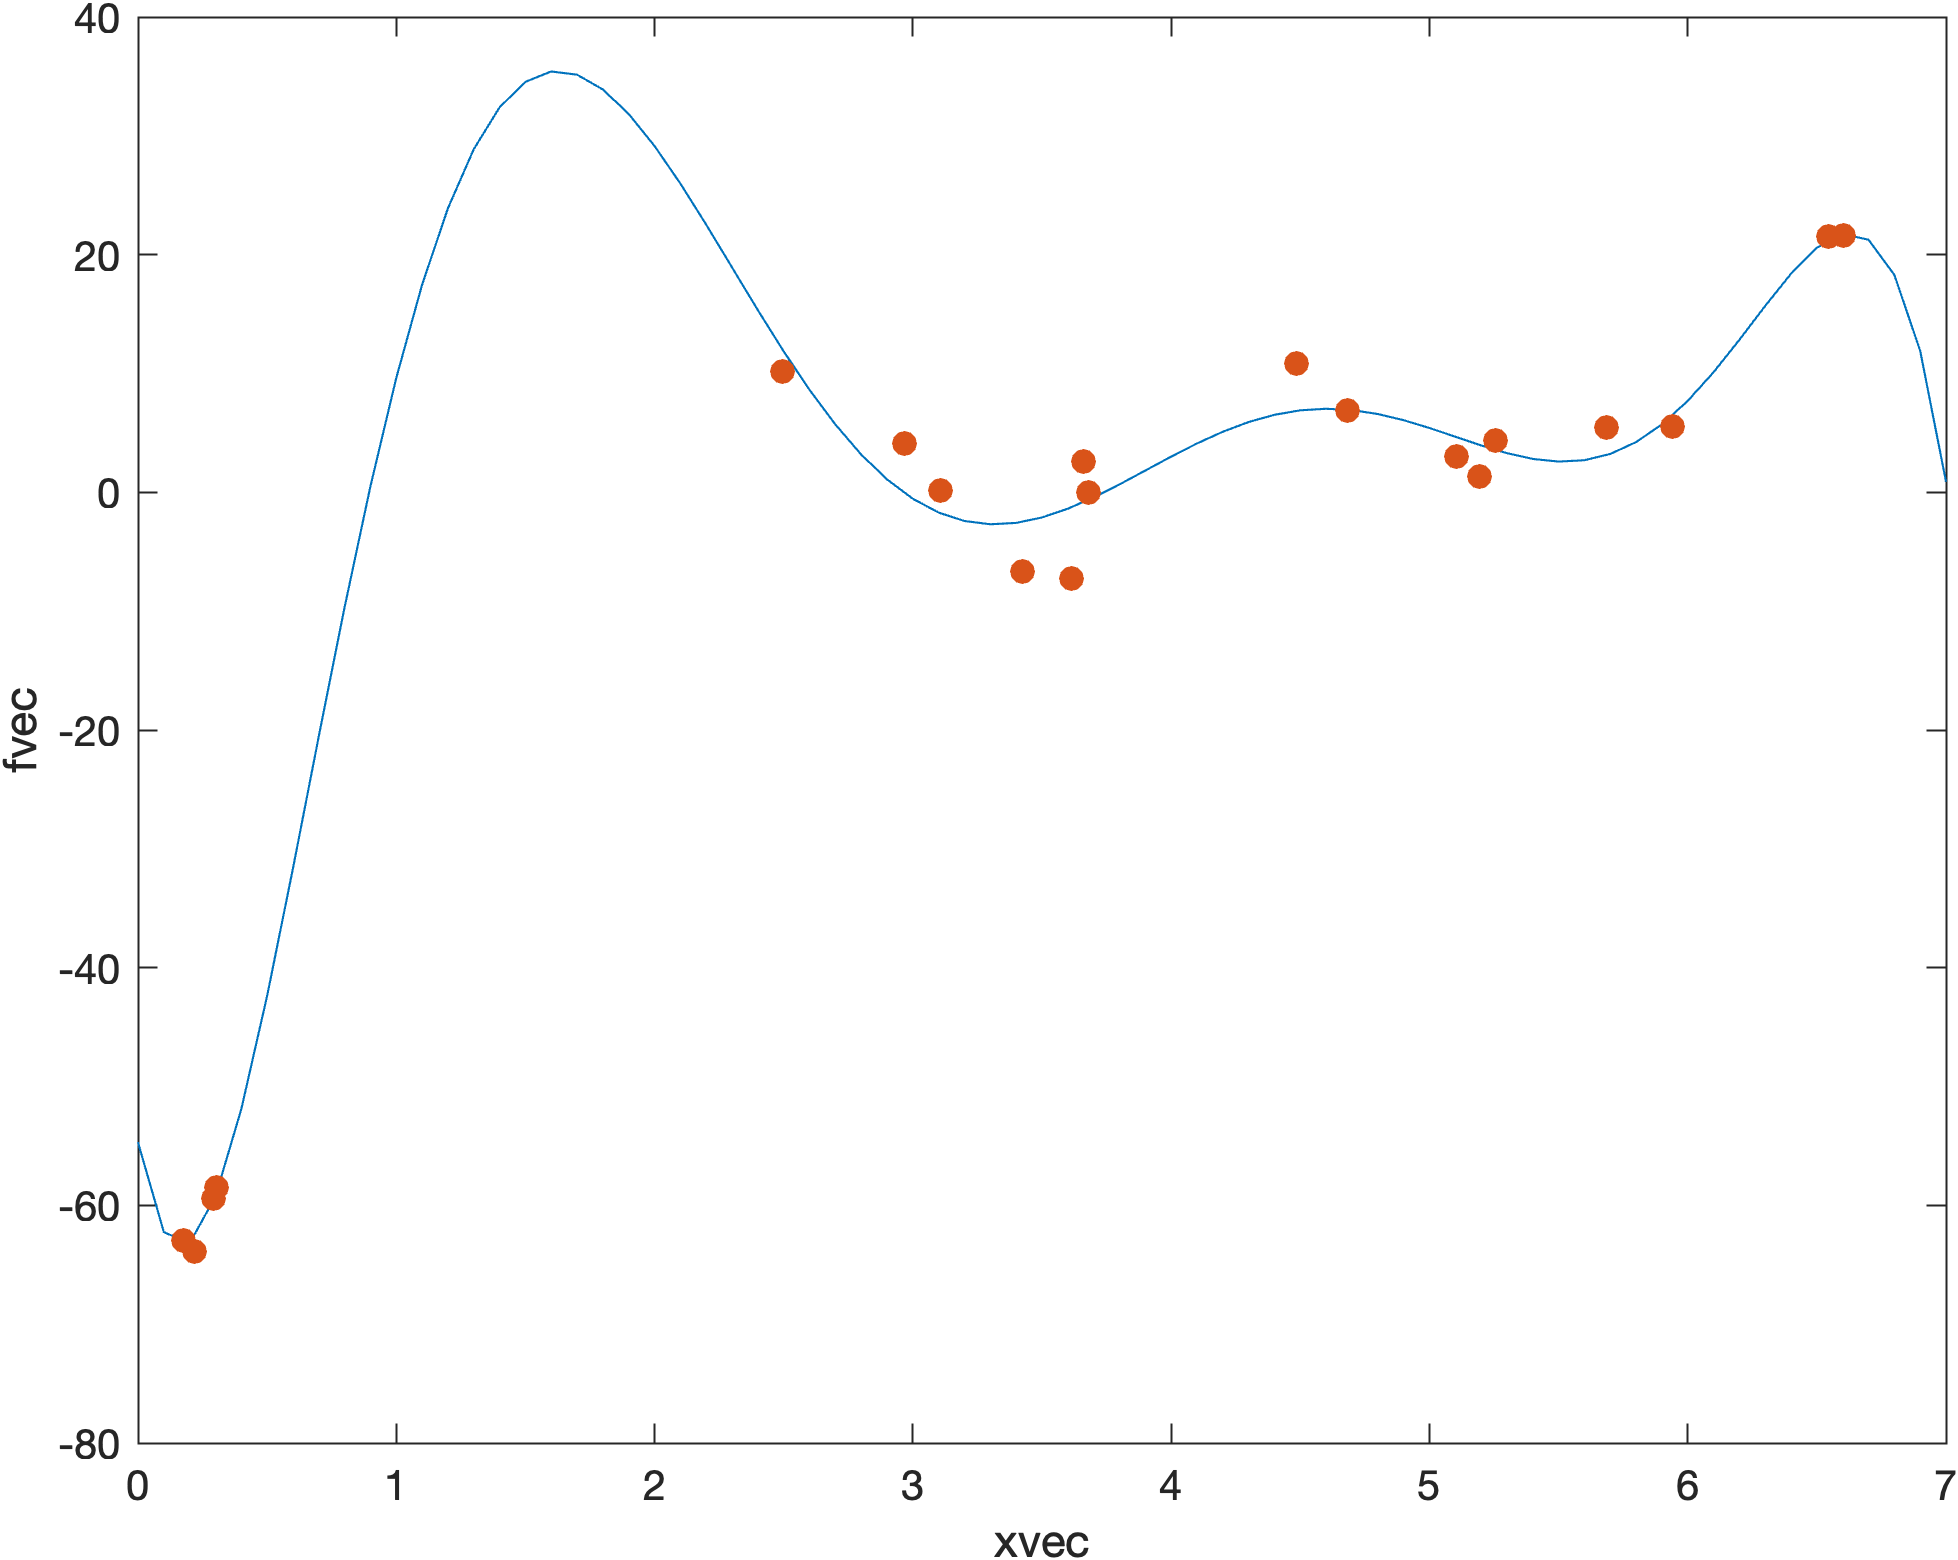
\includegraphics[width=7cm]{leastsquare.png}}
\caption{Optimal polynomial without constraints}
\end{figure}

\begin{minipage}[c]{0.9\textwidth}
\lstinputlisting[language=MatLab]{1a.m}
\end{minipage}

\item For this, we simply create a constrained minimization problem for \ref{ls} with parameters being $c_{i}$ with the constraint that the derivative is non-negative everywhere. Due to Hilbert, non-negativity everywhere is equivalent to the polynomial being a SOS because it's univariate in this case. 
The optimal value comes out to be \texttt{329.348105777} and the optimal polynomial comes out to be $\tt -77.1285656362 + 67.5949992492*x - 10.6081243942*x^2 - 5.07857316587*x^3 + 1.41408502117*x^4 + 0.116990340254*x^5 - 0.0625905841674*x^6 + 0.00476800398802*x^7$. 

\begin{figure}
\centerline{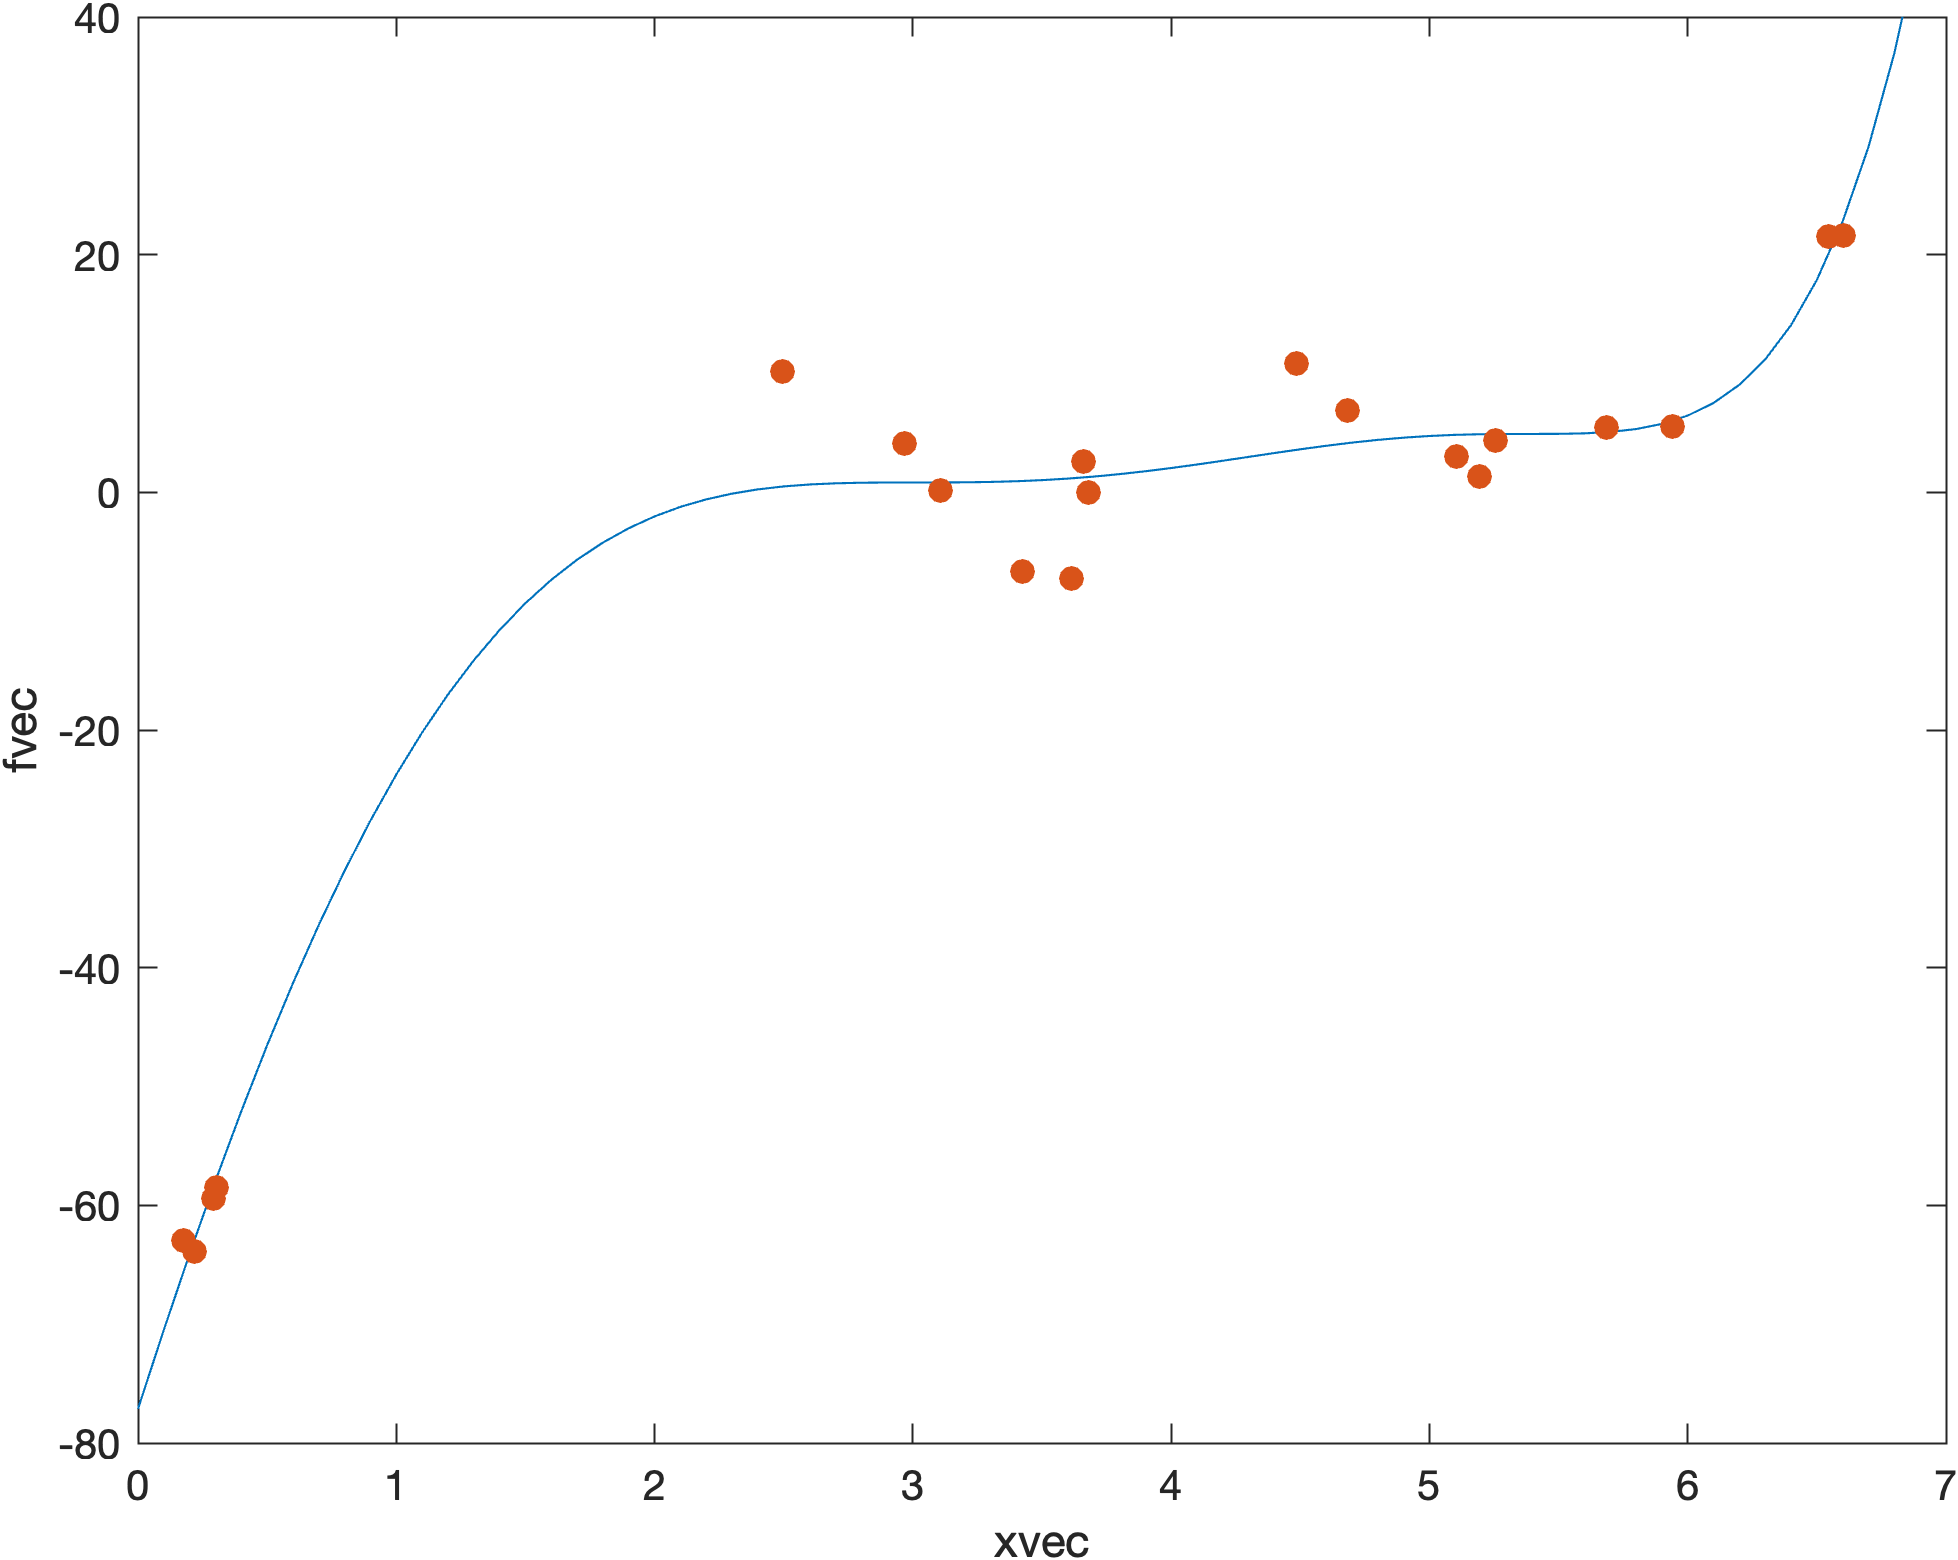
\includegraphics[width=7cm]{leastsquareinc.png}}
\caption{Optimal non-decreasing polynomial}
\end{figure}

\begin{minipage}{0.9\textwidth}
\lstinputlisting[language=MatLab]{1b.m}
\end{minipage}
\end{enumerate}
\item 
\begin{enumerate}[label=(\alph*)]
\item We solve an unconstrained optimization as in \ref{ls2} with parameters being $c_{0},\cdots,c_{15}$. The optimal error came out to be $\eta^{*}=\tt0.607567008796$ and the optimal polynomial came out to be $p^{*} = \tt 0.255317133343-0.969928883268*x_1+2.14288177956*x_2-2.67668839065*x_1^2+8.62632262807*x_1*x_2-13.9522662329*x_2^2+17.0926456078*x_1^3-34.1236189852*x_1^2*x_2+6.32033706645*x_1*x_2^2+21.1619340693*x_2^3-13.2527468384*x_1^4+16.0599795058*x_1^3*x_2+23.1485809245*x_1^2*x_2^2-19.1076202561*x_1*x_2^3-7.511276463*x_2^4$. It's clear from the picture that it's non-convex.

\begin{figure}
\centerline{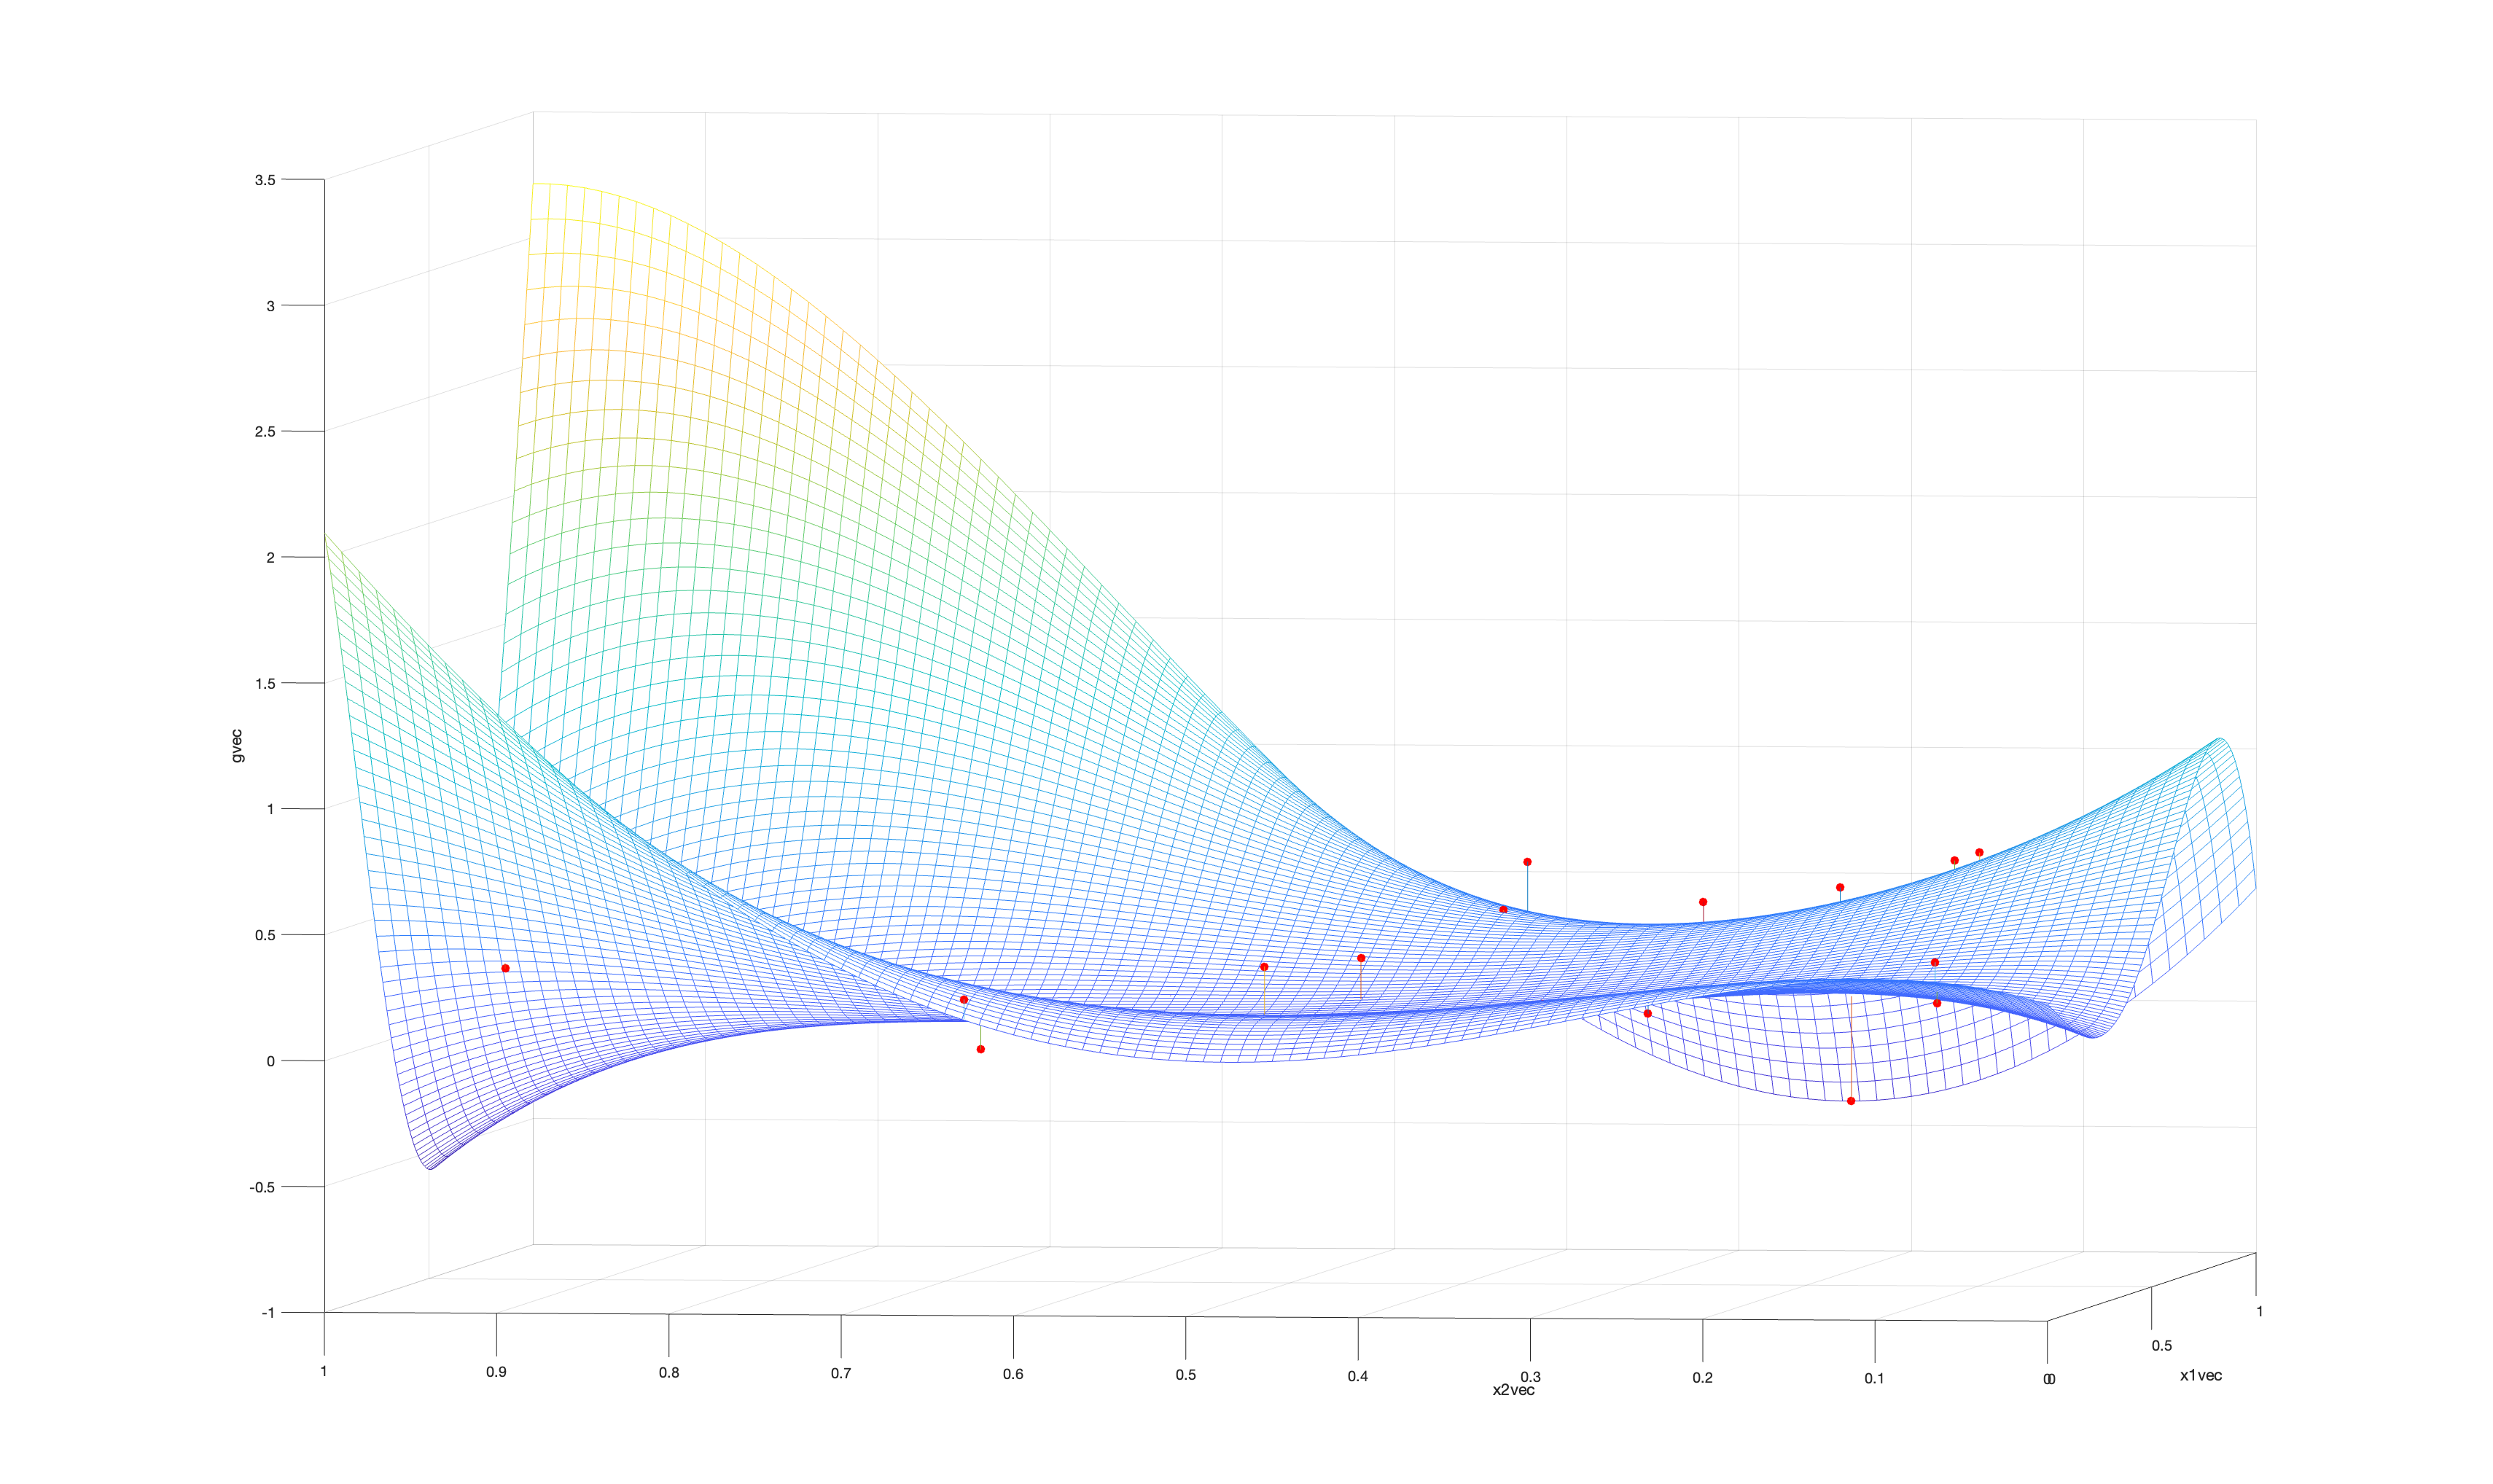
\includegraphics[width=0.9\textwidth]{non-convex.png}}
\caption{Optimal polynomial without constraints}
\end{figure}
\begin{minipage}{0.9\textwidth}
\lstinputlisting[language=MatLab]{2a.m}
\end{minipage}
\item We solve a constrained optimization as in \ref{ls2} with parameters being $c_{0},\cdots,c_{15}$ with the constraints that the Hessian is PSD and the error is at most $1.75\eta^{*}$. The first constraint is enforced by asking that $\begin{bmatrix}s&t\end{bmatrix}H(x_{1},x_{2})\begin{bmatrix}s\\t\end{bmatrix}$ being non-negative for every $x_{1},x_{2},s,t\in\R$ (equivalently SOS because it's a binary quartic in $(x_{1},x_{2},s,t)$). The optimal error came out to be $\tt1.0473433212$ and the optimal polynomial came out to be $p^{*} = \tt 0.573755005423-1.99144979766*x_1-2.21859111356*x_2+5.09138334665*x_1^2+7.0384501806*x_1*x_2+3.92848978664*x_2^2-5.03233518376*x_1^3 - 9.12724553595*x_1^2*x_2-11.6513144747*x_1*x_2^2-2.34405914206*x_2^3+1.91289158409*x_1^4+3.73216359112*x_1^3*x_2+8.86040781842*x_1^2*x_2^2+2.87325038847*x_1*x_2^3 + 1.14003374755*x_2^4$. 


%\begin{minipage}[t]{\linewidth}
\begin{figure}[H]
\centerline{
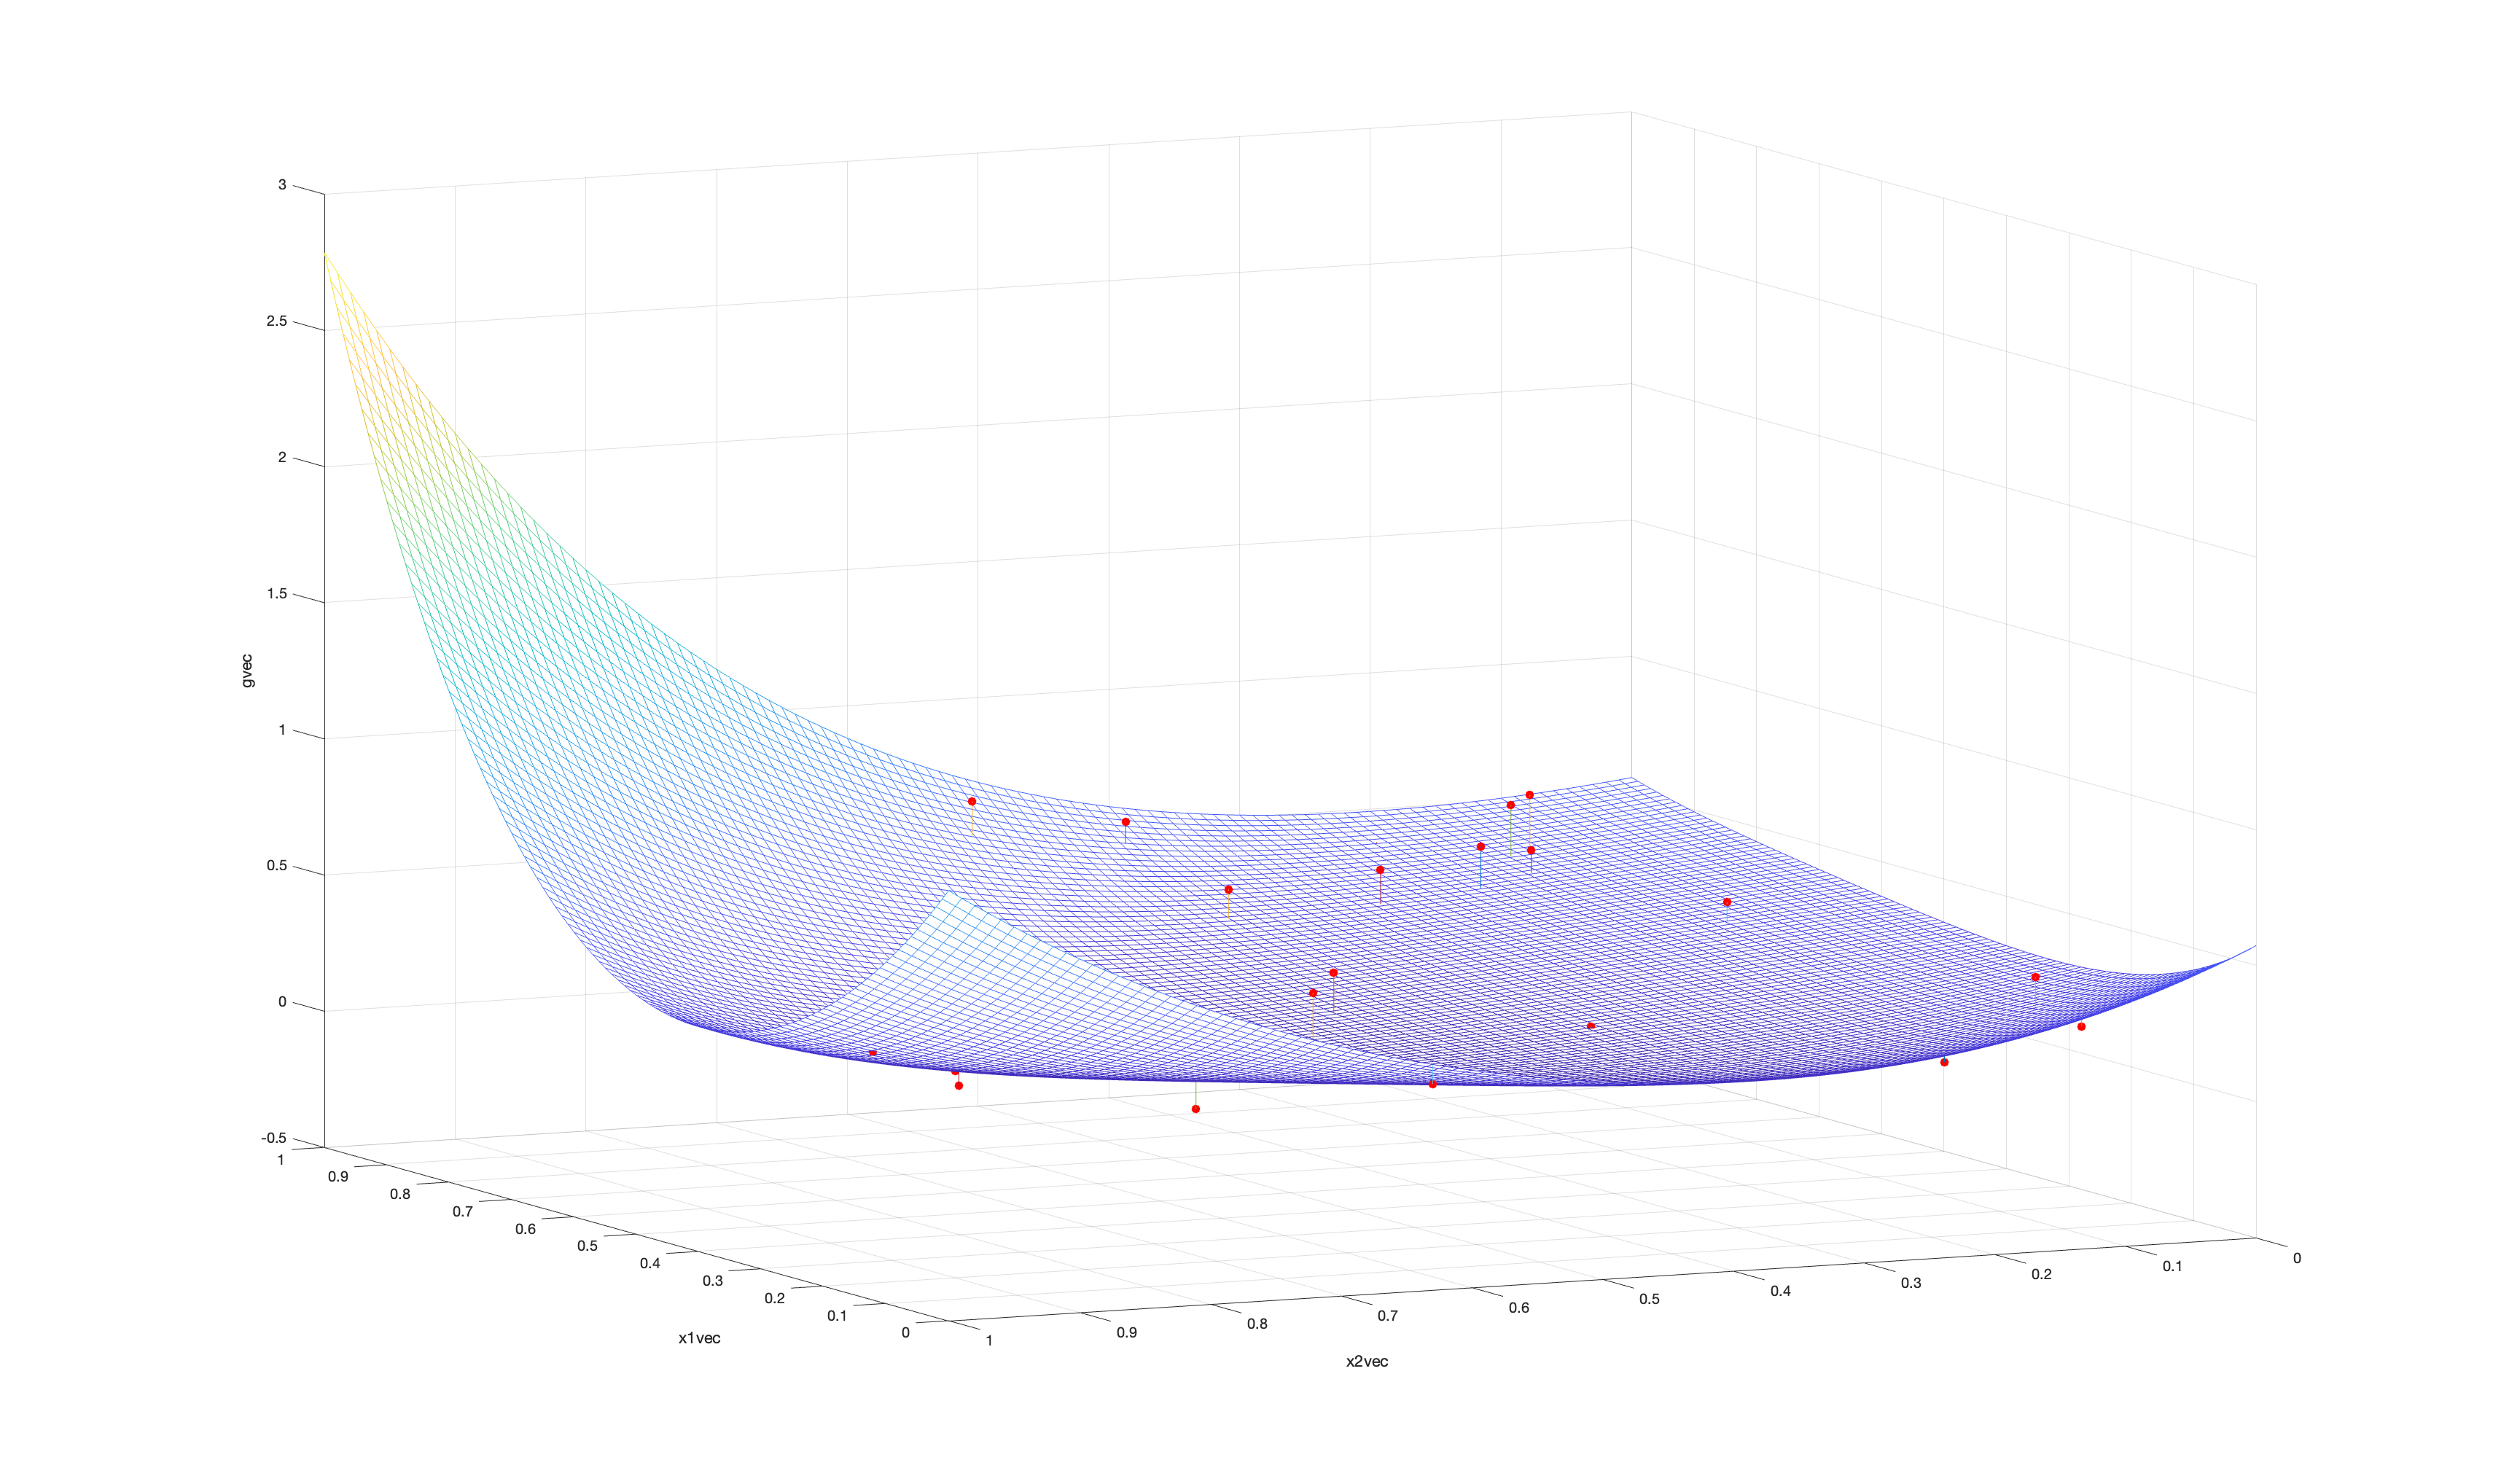
\includegraphics[width=0.7\textwidth]{convex.png}}
\caption{Optimal convex polynomial}
\end{figure}
%\end{minipage}

\begin{minipage}[c]{0.9\textwidth}
\lstinputlisting[language=MatLab]{2b.m}
\end{minipage}
\end{enumerate}
\end{enumerate}



%{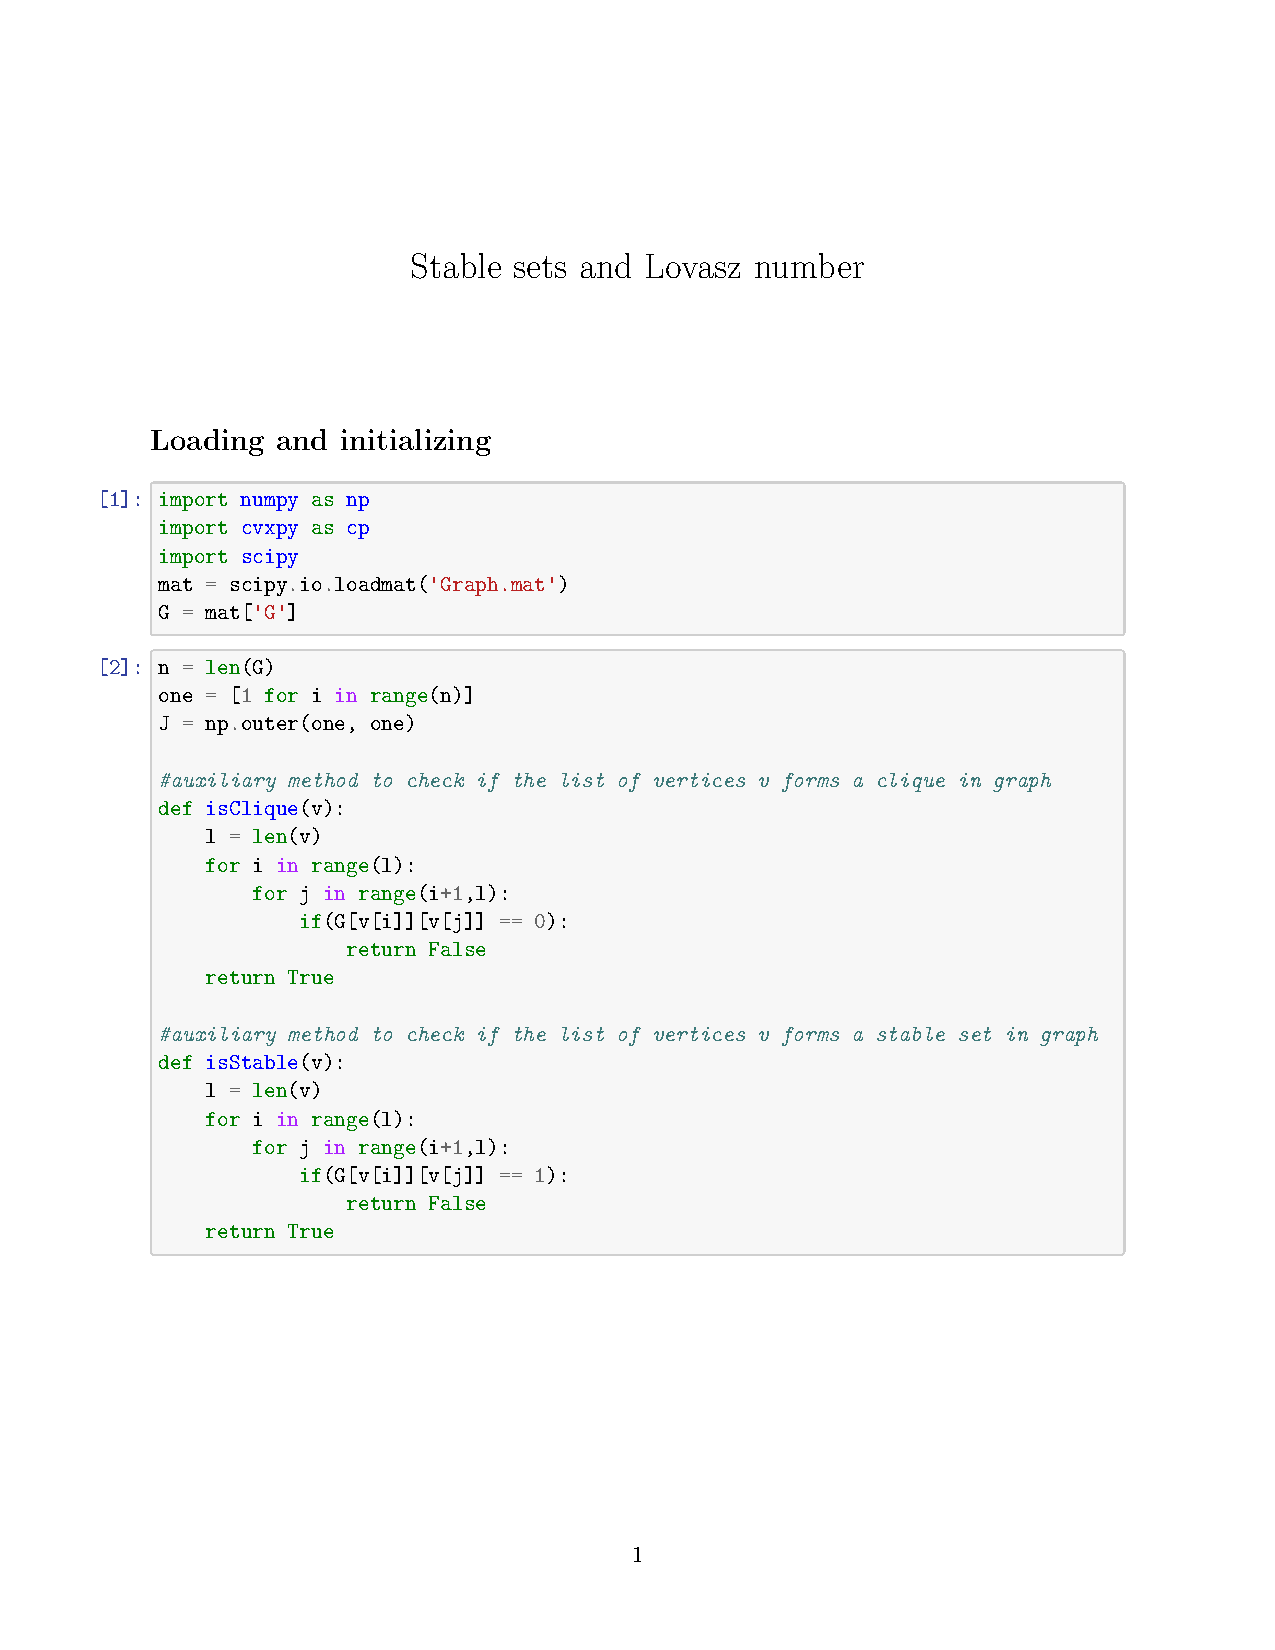
\includepdf[pages=-,pagecommand={\label{pdf:code}}]{graph/graph.pdf}}


\end{document}

